\documentclass{standalone}
\usepackage{tikz}
\usetikzlibrary{patterns, positioning}

\begin{document}
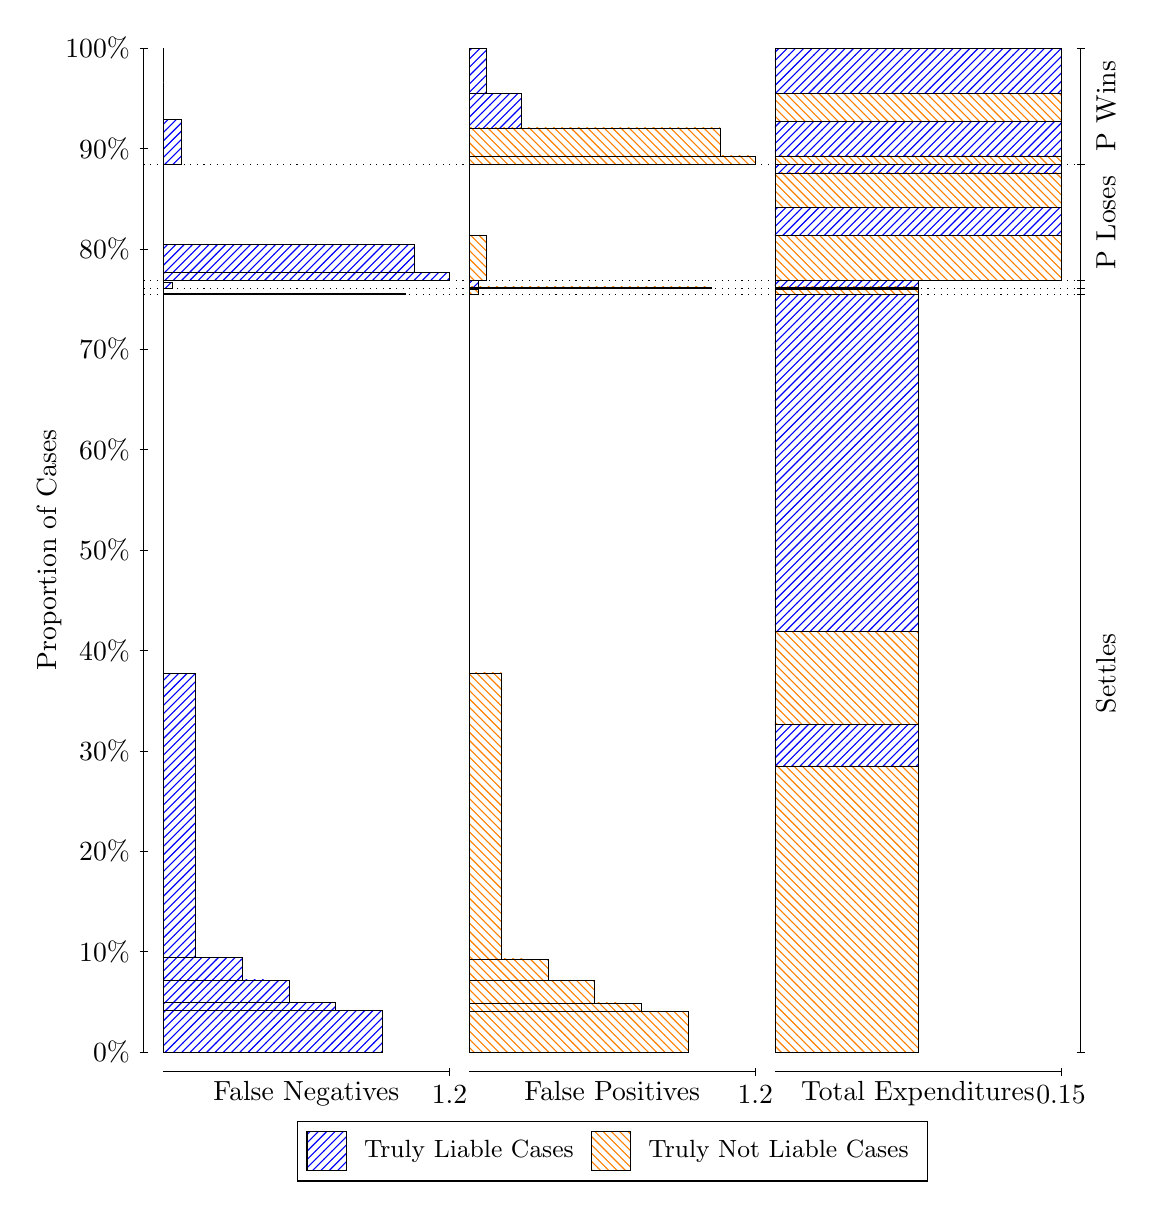
\begin{tikzpicture}
\draw[black, very thin] (1.5,1.75) -- (1.5,14.5);
\node[rotate=90, anchor=center] at (0.3, 8.125) {Proportion of Cases};
\draw[black, very thin] (1.45,1.75) -- (1.55,1.75);
\node[anchor=east] at (1.45, 1.75) {0\%};
\draw[black, very thin] (1.45,3.025) -- (1.55,3.025);
\node[anchor=east] at (1.45, 3.025) {10\%};
\draw[black, very thin] (1.45,4.3) -- (1.55,4.3);
\node[anchor=east] at (1.45, 4.3) {20\%};
\draw[black, very thin] (1.45,5.575) -- (1.55,5.575);
\node[anchor=east] at (1.45, 5.575) {30\%};
\draw[black, very thin] (1.45,6.85) -- (1.55,6.85);
\node[anchor=east] at (1.45, 6.85) {40\%};
\draw[black, very thin] (1.45,8.125) -- (1.55,8.125);
\node[anchor=east] at (1.45, 8.125) {50\%};
\draw[black, very thin] (1.45,9.4) -- (1.55,9.4);
\node[anchor=east] at (1.45, 9.4) {60\%};
\draw[black, very thin] (1.45,10.675) -- (1.55,10.675);
\node[anchor=east] at (1.45, 10.675) {70\%};
\draw[black, very thin] (1.45,11.95) -- (1.55,11.95);
\node[anchor=east] at (1.45, 11.95) {80\%};
\draw[black, very thin] (1.45,13.225) -- (1.55,13.225);
\node[anchor=east] at (1.45, 13.225) {90\%};
\draw[black, very thin] (1.45,14.5) -- (1.55,14.5);
\node[anchor=east] at (1.45, 14.5) {100\%};

\draw[black, very thin] (13.4,1.75) -- (13.4,14.5);
\draw[black, very thin] (13.35,1.75) -- (13.45,1.75);
\node[anchor=west] at (13.35, 1.75) {};
\draw[black, very thin] (13.35,11.368) -- (13.45,11.368);
\node[anchor=west] at (13.35, 11.368) {};
\draw[black, very thin] (13.35,11.45) -- (13.45,11.45);
\node[anchor=west] at (13.35, 11.45) {};
\draw[black, very thin] (13.35,11.545) -- (13.45,11.545);
\node[anchor=west] at (13.35, 11.545) {};
\draw[black, very thin] (13.35,13.022) -- (13.45,13.022);
\node[anchor=west] at (13.35, 13.022) {};
\draw[black, very thin] (13.35,14.5) -- (13.45,14.5);
\node[anchor=west] at (13.35, 14.5) {};

\draw[black, very thin, pattern color=blue, pattern=north east lines] (1.75,1.75) rectangle (4.5306,2.2784);
\draw[black, very thin, pattern color=blue, pattern=north east lines] (1.75,2.2784) rectangle (4.234,2.2802);
\draw[black, very thin, pattern color=blue, pattern=north east lines] (1.75,2.2802) rectangle (3.9374,2.3749);
\draw[black, very thin, pattern color=blue, pattern=north east lines] (1.75,2.3749) rectangle (3.6408,2.3773);
\draw[black, very thin, pattern color=blue, pattern=north east lines] (1.75,2.3773) rectangle (3.3442,2.661);
\draw[black, very thin, pattern color=blue, pattern=north east lines] (1.75,2.661) rectangle (3.0476,2.6646);
\draw[black, very thin, pattern color=blue, pattern=north east lines] (1.75,2.6646) rectangle (2.751,2.9542);
\draw[black, very thin, pattern color=blue, pattern=north east lines] (1.75,2.9542) rectangle (2.4544,2.956);
\draw[black, very thin, pattern color=blue, pattern=north east lines] (1.75,2.956) rectangle (2.1578,6.5548);
\draw[black, very thin, pattern color=orange, pattern=north west lines] (1.75,6.5548) rectangle (1.75,11.368);
\draw[black, very thin, pattern color=blue, pattern=north east lines] (1.75,11.368) rectangle (4.8272,11.382);
\draw[black, very thin, pattern color=orange, pattern=north west lines] (1.75,11.382) rectangle (1.75,11.45);
\draw[black, very thin, pattern color=blue, pattern=north east lines] (1.75,11.45) rectangle (1.8612,11.528);
\draw[black, very thin, pattern color=orange, pattern=north west lines] (1.75,11.528) rectangle (1.75,11.545);
\draw[black, very thin, pattern color=blue, pattern=north east lines] (1.75,11.545) rectangle (5.3833,11.653);
\draw[black, very thin, pattern color=blue, pattern=north east lines] (1.75,11.653) rectangle (4.9384,12.01);
\draw[black, very thin, pattern color=orange, pattern=north west lines] (1.75,12.01) rectangle (1.75,13.022);
\draw[black, very thin, pattern color=blue, pattern=north east lines] (1.75,13.022) rectangle (1.9724,13.595);
\draw[black, very thin, pattern color=orange, pattern=north west lines] (1.75,13.595) rectangle (1.75,14.06);
\draw[black, very thin, pattern color=blue, pattern=north east lines] (1.75,14.06) rectangle (1.75,14.5);
\draw[black, very thin, pattern color=orange, pattern=north west lines] (5.6333,1.75) rectangle (8.4139,2.2685);
\draw[black, very thin, pattern color=orange, pattern=north west lines] (5.6333,2.2685) rectangle (8.1173,2.2699);
\draw[black, very thin, pattern color=orange, pattern=north west lines] (5.6333,2.2699) rectangle (7.8207,2.3716);
\draw[black, very thin, pattern color=orange, pattern=north west lines] (5.6333,2.3716) rectangle (7.5241,2.3739);
\draw[black, very thin, pattern color=orange, pattern=north west lines] (5.6333,2.3739) rectangle (7.2276,2.6572);
\draw[black, very thin, pattern color=orange, pattern=north west lines] (5.6333,2.6572) rectangle (6.931,2.6587);
\draw[black, very thin, pattern color=orange, pattern=north west lines] (5.6333,2.6587) rectangle (6.931,2.6608);
\draw[black, very thin, pattern color=orange, pattern=north west lines] (5.6333,2.6608) rectangle (6.6344,2.9298);
\draw[black, very thin, pattern color=orange, pattern=north west lines] (5.6333,2.9298) rectangle (6.3378,2.9319);
\draw[black, very thin, pattern color=orange, pattern=north west lines] (5.6333,2.9319) rectangle (6.0412,6.5634);
\draw[black, very thin, pattern color=blue, pattern=north east lines] (5.6333,6.5634) rectangle (5.6333,11.368);
\draw[black, very thin, pattern color=orange, pattern=north west lines] (5.6333,11.368) rectangle (5.7446,11.436);
\draw[black, very thin, pattern color=blue, pattern=north east lines] (5.6333,11.436) rectangle (5.6333,11.45);
\draw[black, very thin, pattern color=orange, pattern=north west lines] (5.6333,11.45) rectangle (8.7105,11.466);
\draw[black, very thin, pattern color=blue, pattern=north east lines] (5.6333,11.466) rectangle (5.7446,11.545);
\draw[black, very thin, pattern color=orange, pattern=north west lines] (5.6333,11.545) rectangle (5.8558,12.117);
\draw[black, very thin, pattern color=orange, pattern=north west lines] (5.6333,12.117) rectangle (5.6333,12.557);
\draw[black, very thin, pattern color=blue, pattern=north east lines] (5.6333,12.557) rectangle (5.6333,13.022);
\draw[black, very thin, pattern color=orange, pattern=north west lines] (5.6333,13.022) rectangle (9.2667,13.13);
\draw[black, very thin, pattern color=orange, pattern=north west lines] (5.6333,13.13) rectangle (8.8218,13.487);
\draw[black, very thin, pattern color=blue, pattern=north east lines] (5.6333,13.487) rectangle (6.3007,13.928);
\draw[black, very thin, pattern color=blue, pattern=north east lines] (5.6333,13.928) rectangle (5.8558,14.5);
\draw[black, very thin, pattern color=orange, pattern=north west lines] (9.5167,1.75) rectangle (11.333,5.3836);
\draw[black, very thin, pattern color=blue, pattern=north east lines] (9.5167,5.3836) rectangle (11.333,5.9138);
\draw[black, very thin, pattern color=orange, pattern=north west lines] (9.5167,5.9138) rectangle (11.333,7.0936);
\draw[black, very thin, pattern color=blue, pattern=north east lines] (9.5167,7.0936) rectangle (11.333,11.368);
\draw[black, very thin, pattern color=orange, pattern=north west lines] (9.5167,11.368) rectangle (11.333,11.436);
\draw[black, very thin, pattern color=blue, pattern=north east lines] (9.5167,11.436) rectangle (11.333,11.45);
\draw[black, very thin, pattern color=orange, pattern=north west lines] (9.5167,11.45) rectangle (11.333,11.466);
\draw[black, very thin, pattern color=blue, pattern=north east lines] (9.5167,11.466) rectangle (11.333,11.545);
\draw[black, very thin, pattern color=orange, pattern=north west lines] (9.5167,11.545) rectangle (13.15,12.117);
\draw[black, very thin, pattern color=blue, pattern=north east lines] (9.5167,12.117) rectangle (13.15,12.474);
\draw[black, very thin, pattern color=orange, pattern=north west lines] (9.5167,12.474) rectangle (13.15,12.914);
\draw[black, very thin, pattern color=blue, pattern=north east lines] (9.5167,12.914) rectangle (13.15,13.022);
\draw[black, very thin, pattern color=orange, pattern=north west lines] (9.5167,13.022) rectangle (13.15,13.13);
\draw[black, very thin, pattern color=blue, pattern=north east lines] (9.5167,13.13) rectangle (13.15,13.57);
\draw[black, very thin, pattern color=orange, pattern=north west lines] (9.5167,13.57) rectangle (13.15,13.928);
\draw[black, very thin, pattern color=blue, pattern=north east lines] (9.5167,13.928) rectangle (13.15,14.5);
\draw[black, dotted] (1.5,11.368) -- (13.4,11.368);
\draw[black, dotted] (1.5,11.45) -- (13.4,11.45);
\draw[black, dotted] (1.5,11.545) -- (13.4,11.545);
\draw[black, dotted] (1.5,13.022) -- (13.4,13.022);
\draw[black, very thin] (1.75,1.5) -- (5.3833,1.5);
\node[anchor=north] at (3.5667, 1.5) {False Negatives};
\draw[black, very thin] (5.3833,1.45) -- (5.3833,1.55);
\node[anchor=north] at (5.3833, 1.45) {1.2};

\draw[black, very thin] (5.6333,1.5) -- (9.2667,1.5);
\node[anchor=north] at (7.45, 1.5) {False Positives};
\draw[black, very thin] (9.2667,1.45) -- (9.2667,1.55);
\node[anchor=north] at (9.2667, 1.45) {1.2};

\draw[black, very thin] (9.5167,1.5) -- (13.15,1.5);
\node[anchor=north] at (11.333, 1.5) {Total Expenditures};
\draw[black, very thin] (13.15,1.45) -- (13.15,1.55);
\node[anchor=north] at (13.15, 1.45) {0.15};

\node[black, centered, rotate=90] at (13.72, 6.5591) {Settles};


\node[black, centered, rotate=90] at (13.72, 12.283) {P Loses};
\node[black, centered, rotate=90] at (13.72, 13.761) {P Wins};

\draw (7.449999999999999,1.5) node[draw=none] (baseCoordinate) {};
\begin{scope}[align=center]
        \matrix[scale=0.5, draw=black, below=0.5cm of baseCoordinate, nodes={draw}, column sep=0.1cm]{
            \node[rectangle, draw, minimum width=0.5cm, minimum height=0.5cm, pattern=north east lines, pattern color=blue] {}; &
            \node[draw=none, font=\small] (B) {Truly Liable Cases}; &
            \node[rectangle, draw, minimum width=0.5cm, minimum height=0.5cm, pattern=north west lines, pattern color=orange] {}; &
            \node[draw=none, font=\small] (B) {Truly Not Liable Cases}; \\
            };
\end{scope}

\end{tikzpicture}
\end{document}